\section{Material und Methoden}
%%%%%%%%%%%%%%%%%%%%%%%%%%%%%%%%%%%%%%%%%%%%%%%%%%%%%%%%%%%%%

\subsection{Perfusion der Ratte}
%%%%%%%%%%%%%%%%%%%%%%%%%%%%%%%%%

Beim Versuchstier handelte es sich um eine 280~g schwere, weibliche Spraque-Dawley-Ratte. Diese wurde mittels 0.84~ml Narcoren (0.3~ml/100~g, 16~\% Natrium-Pentobarbital) narkotisiert. Das Narkotikum wurde im 45\degree~Winkel in den unteren Bauchraum (intraperitoneal) injiziert. Die Dosis stellt für das Tier eine starke Überdosis dar, die nach einiger Zeit zum Atemstillstand führt. Nach der Injektion folgte eine kurze Ruhephase für das Tier. Da das Versuchstier nach 5:50 Minuten Ruhephase nicht narkotisiert war, wurden weitere 0.3~ml Narcoren, ein Drittel der ursprünglichen Dosis, injiziert. Nach weiteren 3:20 Minuten, nach dem das Tier vollständig narkotisiert war und keinen Zwischensehnenreflex 

\begin{wrapfigure}{r}{0.5\textwidth}
    \centering
    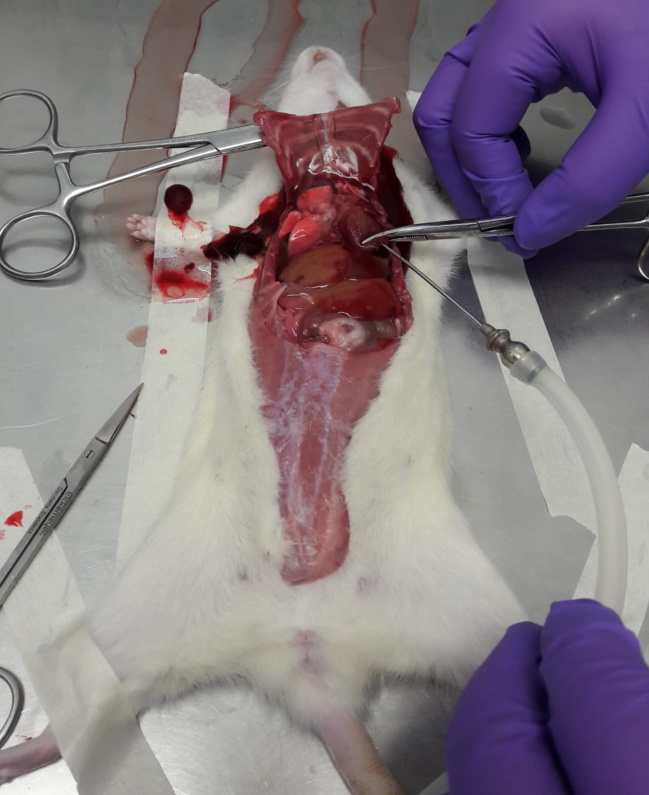
\includegraphics[width=0.47\textwidth]{pictures/Bilder_Jule/Ratte/perfusion.png}
    \caption[Perfusion der Ratte]{\textbf{Perfusion der Ratte.} Der Brustkorb des Tieres ist nach oben hin geöffnet. Mittels Kanüle wird das Blut aus dem Herz-Kreislauf-System gespült.}
    \label{fig:perfusion}
\end{wrapfigure}

mehr zeigte, wurde mit der \textbf{Perfusion} begonnen (Abb.~\ref{fig:perfusion}). Dafür wurde zunächst der Thorax geöffnet um das noch schlagende Herz freizulegen. Die Haut wurde vorsichtig mittig des Bauches von caudal nach rostral geöffnet. Anschließend wurde das Zwerchfell entlang des Rippenbogens aufgetrennt. Das Herzbändchen, sowie die Rippen auf der linken und rechten Seite, wurden durchtrennt. Sobald das Herz freigelegt war, konnte mittels Spritze die linke Herzkammer geöffnet werden um eine Perfusionskanüle (Oliven-Kanüle) einzuführen. Diese wurde mit einer Klemme befestigt. Danach wurde die rechte Herzvorkammer mit einem Schnitt geöffnet. Mit etwa 150~ml 0.01m~PBS (Phosphate-buffered Saline, Raumtemperatur) wurde das Herz-Kreislauf-System unter Verwendung einer Schlauchpumpe vorgespült. Dass sämtliches Blut ausgewaschen ist, ist am blass werdenden Gewebe sichtbar. Bei Ratten mit roten Augen ist dies am Farbwechsel der Augen von rot zu weiß erkennbar. Als dies geschehen war, konnte das Gewebe mittels 350~ml 4~\%igem, eiskaltem Paraformaldehyd fixiert werden. Durch chemische Reaktionen in den Muskeln kann es dabei zu Muskelzuckungen kommen. Die ausreichende Fixierung des Gewebes ist an einer stabilen Kopfposition beim Anheben des Tieres zu erkennen.
\noindent Nach der Fixierung folgte die \textbf{Gehirnentnahme}. Dazu wurde der Kopf des Tieres abgetrennt. Anschließend wurde die Haut dorsal entlang der Mittellinie aufgetrennt. Die die Wirbelsäule umgebene Nackenmuskulatur wurde entfernt. Mit einem Rangeur wurde der Schädelknochen vorsichtig von caudal nach rostral entfernt, bis das Gehirn vollständig freigelegt war. Nachdem alle Knochenrückstände vollständig entfernt wurden, konnte das Gehirn nachfixiert werden. Zur \textbf{Nachfixierung} wurde das Gehirn über Nacht in 4~\%iges Paraformaldehyd gegeben.

\subsection{Färbungen des Gewebes}
%%%%%%%%%%%%%%%%%%%%%%%%%%%%%%%%%%%

In Vorbereitung auf die Färbungen muss das Gehirn in dünne Scheiben geschnitten werden. Um Gewebeschädigungen durch den dazu erforderlichen Gefriervorgang zu vermeiden, ist ein \textbf{Gefrierschutz} erforderlich. Dafür wurde das Gehirn in 20~\%ige Sucroselösung, bestehend aus 20~g Zucker gelöst in jeweils 70~ml Phosphatpuffer, aufgefüllt auf 100~ml, gelegt. Innerhalb dieser Lösung wurde das Gehirn solange aufbewahrt bis es auf den Boden abgesunken war. War dies geschehen, wurde der Vorgang mit 30~\%iger Sucroselösung wiederholt. Da dies einen Tag dauern kann, wurde das Gehirn über das Wochenende in der Lösung gelassen. Zum \textbf{Schneiden} des Gehirns wurde ein Gefriermikrotom verwendet. Um eine bessere Orientierung zu ermöglichen, wurde eine Seite des Cortex mit einem länglichen Schnitt entlang der rostro-caudalen Achse gekennzeichnet. Anschließend wurde das Gehirn in 50~$\upmu$m dicke Scheiben geschnitten, die bis zum Färbevorgang einzeln in mit TBS (Tris-buffered Saline) befüllten Mikroplates im Kühlschrank aufbewahrt wurden. Bei jedem dritten Schritt kam eine unterschiedliche Färbemethode zum Einsatz. Für die Nissl- und Faser-Färbung wurden jeweils vier Schnitte in der richtigen Reihenfolge auf Gelatine Chromalaun beschichteten Objektträgern aufgezogen. Nachdem die Schnitte auf den Objektträgern getrocknet waren, konnte mit dem Färbevorgang begonnen werden. Die mittels immunhistochemischen Nachweises gefärbten Schnitte wurden für den Färbevorgang in zwei Gruppen, a und b, eingeteilt. Dabei wurde jeder zweite Schnitt derselben Gruppe zugeteilt. Erst nach der Färbung wurden die unterschiedlichen Gruppen auf die Objektträger aufgezogen. In den folgenden Abschnitten des Protokolls sind verschiedene, mikroskopische Aufnahmen des gefärbten Gewebes dargestellt. Die \textbf{Namensgebung der Schnitte} setzt sich dabei wie folgt zusammen: Der erste Buchstabe gibt die Färbung an (N: Nissl, F: Faser, I: Immunhistochemisch). Die darauf folgende Zahl beschreibt die Nummer des Objektträgers. Dabei wurden die Schnitte von caudal nach rostral (1-32) aufgezogen. Nach einem Trennstrich folgt die Nummer (1-4) des sich auf dem Objektträger befindenden Schnittes.

\subsubsection{Nissl-Färbung}
%%%%%%%%%%%%%%%%%%%%%%%%%%%%%%

Mittels Nissl-Färbung können Nucleinsäuren, die in den Somata der Zellen enthalten sind, angefärbt werden. In Vorbereitung auf die Nissl-Färbung wurde eine \textbf{Thioninstammlösung} angesetzt. Für diese wurde 1~g Thionin in 10~ml 100~\%igem Alkohol gelöst. Nach 30~min wurden 500~ml destilliertes Wasser hinzu gegeben. Diese Lösung wurde vorsichtig, ohne sie zum Kochen zu bringen, erwärmt. Nach dem sie abgekühlt war und gefiltert wurde, konnte aus der Stammlösung eine Gebrauchslösung gemischt werden. Diese \textbf{Thioningebrauchslösung} bestand aus einer filtrierten Lösung aus 100~ml der Stammlösung, gemischt mit 100~ml destilliertem Wasser. Vor Beginn der Färbung wurden die gut getrockneten Schnitte auf den Objektträgern für 3~min in PBS gegeben. Im Anschluss konnte mit der \textbf{Färbung} begonnen werden. Dafür wurden die Schnitte für 1-2~min in frisch gefilterte Thioninlösung gestellt, solange bis die Schnitte leicht überfärbt waren. Anschließend wurden sie kurz mit 0.01m~mPB abgespült. Die Objektträger wurden für jeweils 3~min in eine aufsteigende Alkoholreihe (50~\%, 70~\%, 90~\%) gegeben. Im folgenden Schritt wurde der Färbegrad der Schnitte kontrolliert. Zu stark gefärbte Schnitte wurden in 96~\%igen Alkohol, gemischt mit 5 Tropfen Eisessig, gegeben. Für zu schwach gefärbte Schnitte wurde die Alkoholreihe in umgekehrter Reihenfolge, und anschließend auch die Färbung, wiederholt. Nach dem alle Schnitte den gewünschten Färbegrad erreicht hatten, wurden die Schnitte für 3~min in 96~\%igen Alkohol, dann zweimal für jeweils 5~min in frischen, 100~\%igen Alkohol gegeben. Danach wurden die Schnitte zweimal für jeweils 10~min in frisches Xylol gelegt. Im Anschluss wurden die noch nassen Schnitte auf den Objektträgern mittels Entellan eingedeckelt. 

\subsubsection{Faser-Färbung}
%%%%%%%%%%%%%%%%%%%%%%%%%%%%%%%

Die Faser-Färbung wurde mittels \textbf{Goldchloridlösung} (0.2~\%) nach Schmued durchgeführt. Mittels dieser Färbemethode werden myelinisierte Fasern angefärbt. Für die Färbelösung wurden 500~ml 0.02m Phosphatpuffer mit 4.5~g Natriumchlorid und 1~g Goldchlorid gemischt. Mit 1~N Natriumhydroxid wurde die Lösung auf einen pH-Wert zwischen 6.8 und 7.0 gepuffert. Zum \textbf{Färben} wurden die trockenen Objektträger mitsamt den Schnitten in die Goldchloridlösung gestellt. Nach etwa 30~min wurden die Schnitte unter dem Mikroskop kontrolliert. Nach dem die Schnitte ausreichend gefärbt waren, dies kann bis zu 1~h dauern, wurden sie in 0.01m~PBS gespült. Danach wurden die Objektträger für 5~min in 2.5~\%ige Natriumthiosulfatlösung gegeben. Im Anschluss wurden sie dreimal für jeweils 5~min in 0.01m PBS gewaschen. Entwässert wurden die Schnitte anschließend ein einer aufsteigenden Alkoholreihe (50~\%, 70~\%, 90~\%, 96~\%, 100~\%, 100~\%). Danach wurden die entwässerten Gehirnschnitte jeweils für 10~min in frisches Xylol gelegt. Im Anschluss wurden sie mit Entellan eingedeckelt.

\subsubsection{Immunhistochemische Färbung}
%%%%%%%%%%%%%%%%%%%%%%%%%%%%%%%%%%%%%%%%%%%%

Die immunhistochemische Färbung dient zum Nachweis catecholaminerger Neurone. Zu den catecholaminergen Stoffen gehören Adrenalin, Noradrenalin, Dopamin, sowie deren Derivate. Alle drei primären Catecholamine werden ausgehend von der Aminosäure Tyrosin synthetisiert \textsuperscript{\cite[Kap.~13]{kandel2013principles}}. An der Synthese sind fünf Enzyme beteiligt. Eines dieser Enzyme, die Tyrosin-Hydroxylase, dient als Grundlage dieses Nachweises. Es lässt sich im Soma und den in den Axontermini catecholaminerger Nervenzellen auffinden. Um dieses Enzym in Gewebe sichtbar zu machen, wurde hier die sogenannte \textbf{ABC-Methode} angewendet. Dies ist ein indirektes Färbeverfahren, das dopaminerg-aktive Regionen (Catecholamin) erkennbar macht. Dazu wurden zwei unterschiedliche Antikörper verwendet. Zum einen ein primärer Antikörper, der direkt an das Enzym Tyrosin-Hydroxylase bindet und ein sekundärer, biotinylierter Antikörper, der sich wiederum an den primären Antikörper anheftet. An das biotinylierte Ende des sekundären Antikörpers binden Avidin-Biotin-Complexe, die Meerrettichperoxidase-Moleküle (HRP) enthalten. Wird nun das farblose 3,3'-Diaminobenzidin-Tetrahydrochlorid (DAB) hinzugegeben, oxidiert der Komplex zu einem bräunlichem Produkt \textsuperscript{\cite{burry2009immunocytochemistry}}. Die Durchführung des Nachweises kann in mehrere Schritte unterteilt werden. Vor dem ersten Schritt wurden die Schnitte, die sich in Microplates befanden, mit TBS Puffer gewaschen. Der erste Schritt der Färbung wird als \textbf{Quenching} bezeichnet. Hierbei wurden die Schnitte in TBS-Puffer zusammen mit 0.3~\%~igem Wasserstoffperoxid (0.3~ml 30~\%~iges H$_{2}$0$_{2}$ in 100~ml PBS) gegeben. Damit sollte eine nicht-spezifische Hintergrundfärbung durch endogene Peroxidasen vermieden werden. Das zugegebene Wasserstoffperoxid stoppt endogene Peroxidasen im Gewebe, die eventuell eine falsch-positive Reaktion mit DAB (letzter Schritt) hervorrufen könnten \textsuperscript{\cite{burry2009immunocytochemistry}}. Anschließend wurden die Schnitte wiederum in TBS gewaschen und es folgte der zweite Schritt, das \textbf{Blocken} unspezifischer Bindungen und die \textbf{Permeabilisierung} der Zellmembran. Dies wurde durch Zugabe eines Blockers bestehend aus 9~ml Goat-Serum und 1~ml Carrier ermöglicht. Der Carrier wiederum setzte sich aus 150~ml TBS, 3~ml Goat-Serum und 2.25~ml 20~\%~igem Triton X zusammen. Um nicht-spezifische Protein-Protein-Interaktion zwischen Antikörpern und Proteinen zu unterbinden, muss sich vor Zugabe des ersten Antikörpers ein blockendes Protein kompetitiv mit den unspezifischen Bindungsstellen verknüpfen. Der Antikörper bindet an die sogenannten \textbf{Fc-Rezeptoren} im Gewebe. Diese sind auf Makrophagen und vielen anderen immunologischen Zellen im Gewebe zu finden und könnten daher jeden Antikörper, der während der Färbung hinzugeben wird, binden. Das Triton-X ist ein nicht-ionisches Tensid und fungiert als Detergent. Seine Zugabe führt zu einer Auflockerung der Zellmembran, sodass die Antikörper in die Zelle eindringen und intrazellulär binden können \textsuperscript{\cite{burry2009immunocytochemistry}}. Nach dem Blocken erfolgte der dritte Schritt mit Zugabe des \textbf{primären Antikörpers}. Dieser bestand aus dem Antikörper r-a-TH (rabbit-anti-Tyrosin-Hydroxylase), der 1:500 mit dem Carrier verdünnt wurde (20~$\upmu$l AK in 9980 ~$\upmu$l Carrier). Der primäre Antikörper besitzt eine \textbf{Fc-Region} und eine \textbf{Fab-Region}. Die Fab-Region des primären Antikörpers bindet an das Epitop der Tyrosin-Hydroxylase \textsuperscript{\cite{burry2009immunocytochemistry}}. Das Gemisch wurde unter ständigem schütteln über Nacht in den Kühlschrank gestellt. Am zweiten Tag wurden die Schnitte zunächst mit TBS-Puffer gewaschen, bevor dann im vierten Schritt der \textbf{sekundäre Antikörper} hinzu gegeben wurde. Der Sekundärantikörper ist biotinyliertes Goat-a-r (Goat-anti-rabbit), das 1:1000 in Carrier gemischt wurde (10~$\upmu$l AK mit 9990~$\upmu$l Carrier). Er bindet mit seiner Fab-Region an die Fc-Region des primären Antikörpers \textsuperscript{\cite{burry2009immunocytochemistry}}. Nach einer Stunde wurde der Rest mit PBS-Puffer ausgewaschen und es erfolgte der fünfte Schritt, die Zugabe des \textbf{Avidin-Biotin-Complex (ABC)}. Das ABC-Kid wurde 30~min zuvor angesetzt und bestand aus  100~$\upmu$l Avidin, 100~$\upmu$l Biotin und 10~ml des Carriers PBN. Dieser Carrier wiederum setzt sich aus 12.5~ml 0.2~M Phosphatpuffer, 7.3~g Natriumclorid und 250~ml destilliertem Wasser zusammen. Am Biotin befinden sich zusätzlich zahlreichen HRP-Moleküle, die sich unter der Zugabe von Avidin in Komplexen anreichern. Dieser Komplex lagert sich nun am biotinyliertem Sekundärantikörper an \textsuperscript{\cite{burry2009immunocytochemistry}}. Der restliche ungebundene Antikörper wurde nach 60~min durch Waschen in TBS entfernt. Anschließend folgte der letzte Schritt, die \textbf{DAB-Reaktion}, die auch die charakteristische braune \textbf{Färbung} erzeugt. Für diese Reaktion wurden 10~mg DAB mit 20~ml filtriertem TBS gemischt. Kurz vor Gebrauch wurde zusätzlich noch 9~$\upmu$l Wasserstoffperoxid hinzu gegeben. Das farblose DAB wird von der an den AB-Komplex gebundene Meerrettich-Peroxidase (HRP) zu einem braunen Produkt oxidiert \textsuperscript{\cite{burry2009immunocytochemistry}}. Dieser Färbegrad wurde kontinuierlich kontrolliert und als die Schnitte ausreichend gefärbt waren, wurde die Reaktion mit TBS-Puffer gestoppt. Anschließen wurden die Schnitte sortiert, auf Objektträger aufgezogen und über Nacht getrocknet. Am dritten Tag wurden die Schnitte dann zunächst über eine aufsteigende Alkoholreihe (50~\%, 70~\%, 80~\%, 90~\%, 96~\%, 2~x~100~\%) entwässert. Im Anschluss wurden die Objektträger zweimal für 10~min in frisches Xylol gestellt und danach mit Entellan eingedeckelt.  


\subsection{Mikroskopie}
%%%%%%%%%%%%%%%%%%%%%%%%%%%%%%%%%%%%%%%%%%%

Die Bilder der einzelnen Färbungen wurden mit einem Mikroskop der Firma Zeiss aufgenommen und mit dem Programm 'Axio Vision' (AxioVs40 4.8.2.0 \textsuperscript{\textcopyright} 2006-2010, Carl Zeiss MicroImaging GmBH) an einem Aufnahmecomputer bearbeitet. Mit diesem Programm konnten Panoramabilder erstellt werden und die quantitative Analyse der Kerngebiete und Zellen des catecholaminergen Systems (Kap.~\ref{sec:immu}) berechnet werden.
